\chapter{Memory Analysis}
To get a better insight on how Hive uses memory, I needed to build a basic model when and why Hive's reserved memory grows. During my work, I mainly focused on HiveServer2. The first step toward the model building was to get basic knowledge about Hive's code base and the query compilation process. The query life cycle mentioned in the previous chapter helped, but I had to find those steps in the code. If I have these points I am able to start measuring and maybe find some memory wastes.

\section{Finding the measuring points}
Hive has around 2 million lines of code so locating the main steps of the query processing was challenging. 

As a starting point, the user enters a query in the client. At this point, I run Hive locally, so the simplest way for submitting queries against Hive was using Beeline command line client. HS2 gets the query through its Thrift interface. After this, the query goes to the \textit{Driver} class, which is the main class for executing queries.

The Driver has two methods that are important for me: run and runInternal. The run method gets called first, which basically just delegates to the runInternal method. These two functions return with a CommandProcessorResponse, once the compilation and execution are done. 

\noindent The runInternal does the two main steps:
\begin{itemize}
	\item Driver.compile: gets the command string and parses, analyses the query and generates the execution plan.
	\item Driver.execute: gets the execution plan and executes it on a specific engine (MapReduce, Spark or TEZ).
\end{itemize}

\subsection{Compile}
The first step of the compilation is the parsing. It takes a string and returns an Abstract Syntax Tree (AST or the Parse Tree).

\begin{lstlisting}
public int compile(String command, ...) {
...
	ASTNode tree;
	try {
		tree = ParseUtils.parse(command, ctx);
	} catch (ParseException e) {
...
}
\end{lstlisting}
\subsubsection{Semantic Analyzis}
After the AST is generated, the compile process will continue with the semantic analyzer. The type of the analyzer will depend on the query type we are running. For SELECT and INSERT the SemanticAnalyzer class is used. 

\begin{lstlisting}
public int compile(String command, ...) {
...
	BaseSemanticAnalyzer sem = SemanticAnalyzerFactory.get(queryState, tree);
...
	sem.analyze(tree, ctx);
...
}
\end{lstlisting}

The SemanticAnalyzer class is the main phase during compilation. It checks for semantic errors, fetches metadata from Metastore, generates and optimizes the query plan. The analyze method of the BaseSemanticAnalyzer is called from the Driver's compile method, and it delegates the call to the corresponding Analyzer. From now on, I will write about the SemanticAnalyzer class and its phases (which is executed for SELECTS and INSERTS.

\begin{lstlisting}
void analyzeInternal(ASTNode ast, PlannerContext plannerCtx) {
	//(1)
	if (!genResolvedParseTree(ast, plannerCtx)) {
		return;
	}
	//(2)
	Operator sinkOp = genOPTree(ast, plannerCtx);
	...
	//(3)
	...
	resultSchema = convertRowSchemaToViewSchema(...);
	...
	//(4)
	Optimizer optm = new Optimizer();
	... = optm.optimize();
	...
	//(5)
	TaskCompiler compiler = TaskCompilerFactory.getCompiler(conf, pCtx);
	compiler.compile(pCtx, rootTasks, inputs, outputs);
	...
}
\end{lstlisting}

\begin{enumerate}
	\item Fetches metadata and fill the Parse Tree with it so it becomes a Resolved Parse Tree.
	\item The Operation Tree gets created which will contain operators that process data read from the table. This tree is called by the Map and Reduce methods.
	\item The semantic analyzer will deduce the schema of the result set from the row schema
	\item A logical optimization is done on the Operator Tree. There are two types of optimization: one that transforms the Operator Tree (like removing unnecessary operations) and one that does not (predicate pushdown, vectorization \etc).
	\item Physical optimization and translation to the target execution engine take place. The output of this stage is the query plan. It can optimize the tree according to the engine used. For example in MR, common join can be translated to map-side join, if one of the tables is small enough to fit into the memory of the map nodes.
\end{enumerate}

\begin{lstlisting}
public int compile(String command, ...) {
	...
	sem.validate();
	...
}
\end{lstlisting}

After the semantic analysis is completed, the Driver will validate the plan. When it completes, the compilation ends and Hive will continue with the execution.

\clearpage
\section{Measure the memory of HiveServer2}
If I want to measure the memory usage of Hive, I need a something to create and analyze heap dumps and generate memory statistics. There are several tools to choose from. In this section, I will present the tools I considered and the method I used to get a better understanding of HS2 memory patterns.

\subsection{Tools for generating heap dumps and statistics}
For creating heap dumps and statistics of the memory, I decided to use a command line tool. In contrast of a UI tool, it has the benefits to generate heap dumps and statistics automatically. 

\subsubsection{jmap}
\textit{jmap} \cite{jmap} can be used to obtain heap dumps and histograms from a running java process.

To gather information about a running Java program we need its process ID (PID). Using this we can easily create the heap dump with the \textit{-dump} option. If we do not want to analyze large heap dumps, just to get the objects that reserve the most memory, we can use the \textit{-histo} option. It will print a histogram of the heap, containing each Java class, the number of objects and memory sizes per class.

\subsubsection{jcmd}
\textit{jmap} would have been a perfect choice for measuring memory. However, it is recommended to use the latest utility, which is called \textit{jcmd} \cite{jcmd}. It has enhanced diagnostics capability and its perfomance overhead is reduced. 

The usage of jcmd is similar to jmap. For creating heap dumps we can use \textit{jcmd <PID> GC.heap\_dump}. If we want to obtain class histogram we can do that with the \textit{jcmd <PID> GC.class\_histogram} command. With the \textit{jcmd <PID> GC.heap\_info} command we can gather basic information of the heap: \eg young and old memory of the process.

I decided to use jcmd in my future work to gather memory information automatically and generate heap dumps at the measuring points identified in the previous section.

\subsection{Tools for analysing heap dumps}
Creating heap dumps with a CLI tool is easier, however analysing those requires a tool with user interface. 

\subsubsection{YourKit}
\textit{YourKit} provides great analysing capabilities for heap dumps. We can use it for profiling local or remote Java applications. It has controllable overhead. Although, it is a great tool for profiling Java applications, it is a commercial software and only has 15 days of free licence.

\subsubsection{VisualVM}
\textit{VisualVM} provides a great visual interface for profiling Java applications and browsing heap dumps. It offers multiple views for analysing them. We can get the summary of the dump which contains the total bytes, classes and objects. 

With the "classes view" we can get information about the reserved memory and number of instances for each class. We can calculate the retained memory, which is the memory that would be freed if the objects would be garbage collected.

\subsubsection{JXRay}
JXRay \cite{jxray} is a memory analysis tool for Java applications. It creates a HTML report of a given heap dump. It can automatically detect common problems, like data duplication or non-optimal usse of data stuctures. 

JXRay can give us a compact report, even if the heap dump analyzed is 10's of GB. It can calculate how much memory taken by a collection internal representation and their workload, since JXRay knows about the internal representation of common java collections (HashMap, ArrayList \etc).

\begin{figure}[H]
	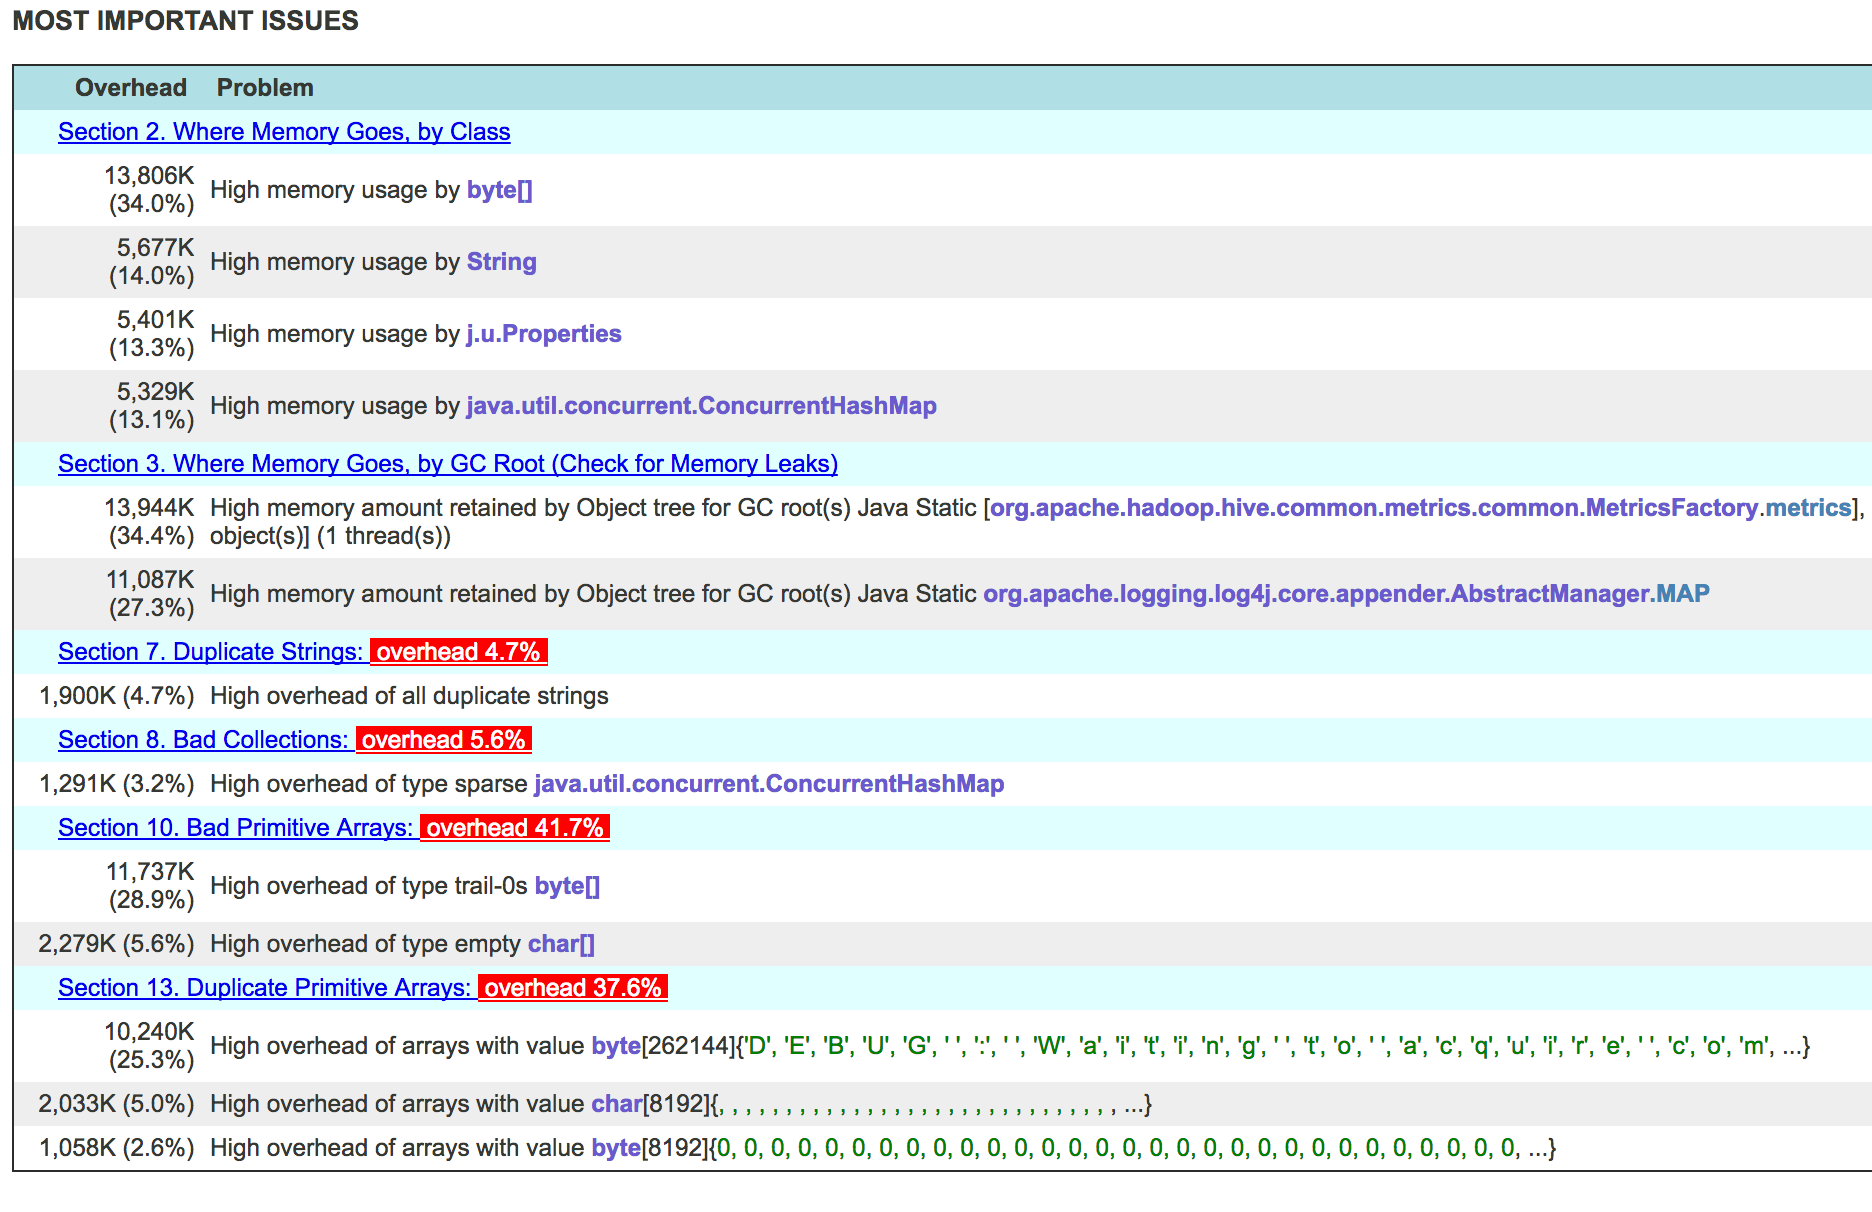
\includegraphics[width=150mm, keepaspectratio]{figures/jxray_sample.png}
	\centering
	\caption{Sample JXRay report summary}
\end{figure}

\subsubsection{The selected tool}
I decided to use VisualVM for visual memory analysis since it has great capabilities for summarizing the most important information about a heap dump and with its help, I am able to walk through the memory tree easily.

During my work, I also used JXRay, since it can automatically detect the most common memory problems and give me an overview of the possible issues a Java application has.

\clearpage
\subsection{Creating the code to measure memory}
With the available tools I am able to generate heap dumps really easily. However, to get a model how Hive uses the memory, I should gather statistics and heap dumps at certain points of the query execution. Clearly, it is not possible by hand. Thus, I needed to create a class in Hive's codebase and integrate the sampling in the identified points found in the previous section.

In order to use jcmd from Java, I needed a way to execute a terminal command from code. With the \textit{ProcessBuilder} java class I'm able to create operating system processes with the given attributes. The \textit{Runtime.exec()} method would do the same, but using this command is discouraged. 

Now that I can run a command line tool from Java, I will need the process ID of HiveServer2. Since Hive uses Java 8, I cannot use the new Process API that Java 9 provides. With the help of the \textit{ManagementFactory} class, we can get the managed bean of the runtime system of the JVM. It will return a class implementing the \textit{RuntimeMXBean} interface. The name of the running JVM contains the ID of the process. With the \textit{RuntimeMXBean.getName()} method, I was able to get the PID of HiveServer2. The method will return a string in a format of: \textit{pid@hostname}. Using the split method we can get our application's process ID.

To avoid code duplication I created a method for getting the ProcessBuilder which contains the given command and the PID for HiveServer2 is already set.

\begin{lstlisting}
private ProcessBuilder getProcessBuilder(String subCommand){
	ProcessBuilder builder = new ProcessBuilder();
	//Get own pid
	String pid = ManagementFactory.getRuntimeMXBean().getName().split("@")[0];
	builder.command("sh", "-c", String.format("jcmd %s %s", pid, subCommand));
	return builder;
}
\end{lstlisting}

Using the \textit{getProcessBuilder} function, it is really simple to run a terminal command. For example, getting information about the state of the heap or creating a heap dump will look like this:

\begin{lstlisting}
...
 process =  getProcessBuilder("GC.heap_info").start();
 ...
 getProcessBuilder("GC.heap_dump " + path).start();
\end{lstlisting}

\subsubsection{Parsing result}
I am able to create detailed statistics about the current memory state at certain phases of the query. As a first approach, I decided to just use \textit{GC.heap\_info} to see how memory usage looks like at different stages, not caring how much memory is reserved by each class. However, if we look at the result of the \textit{jcmd <PID> GC.heap\_info}, it will look quite messy, and hides the most important details, especially if we have 15 result for each query. An example how it looks:

\begin{lstlisting}
21566:
PSYoungGen total 1395200K, used 27419K [0x000000076ab00000, 0x00000007c0000000,
0x00000007c0000000)
eden space 1392640K, 1% used
[0x000000076ab00000,0x000000076c5c6c70,0x00000007bfb00000)
from space 2560K, 0% used [0x00000007bfd80000,0x00000007bfd80000,0x00000007c0000000)
to space 2560K, 0% used [0x00000007bfb00000,0x00000007bfb00000,0x00000007bfd80000)
ParOldGen total 1046528K, used 14704K [0x00000006c0000000, 0x00000006ffe00000,
0x000000076ab00000)
object space 1046528K, 1% used
[0x00000006c0000000,0x00000006c0e5c058,0x00000006ffe00000)
Metaspace used 48314K, capacity 48612K, committed 49280K, reserved 1093632K
class space used 5359K, capacity 5440K, committed 5504K, reserved 1048576K
\end{lstlisting}

I only need certain values: allocated young and old memory, and a total memory which is the sum of the young and old values. I created a function called getResult which will read the result from a given process and return in string format. The returned string will look like above, so parsing is needed if I want to gather the important details.

To do this, I made a function (printResultToCSV) which will parse the given string, and print the results to a csv file in a table like format, where the first line is the query, and the columns are the different stages.

\begin{figure}[H]
	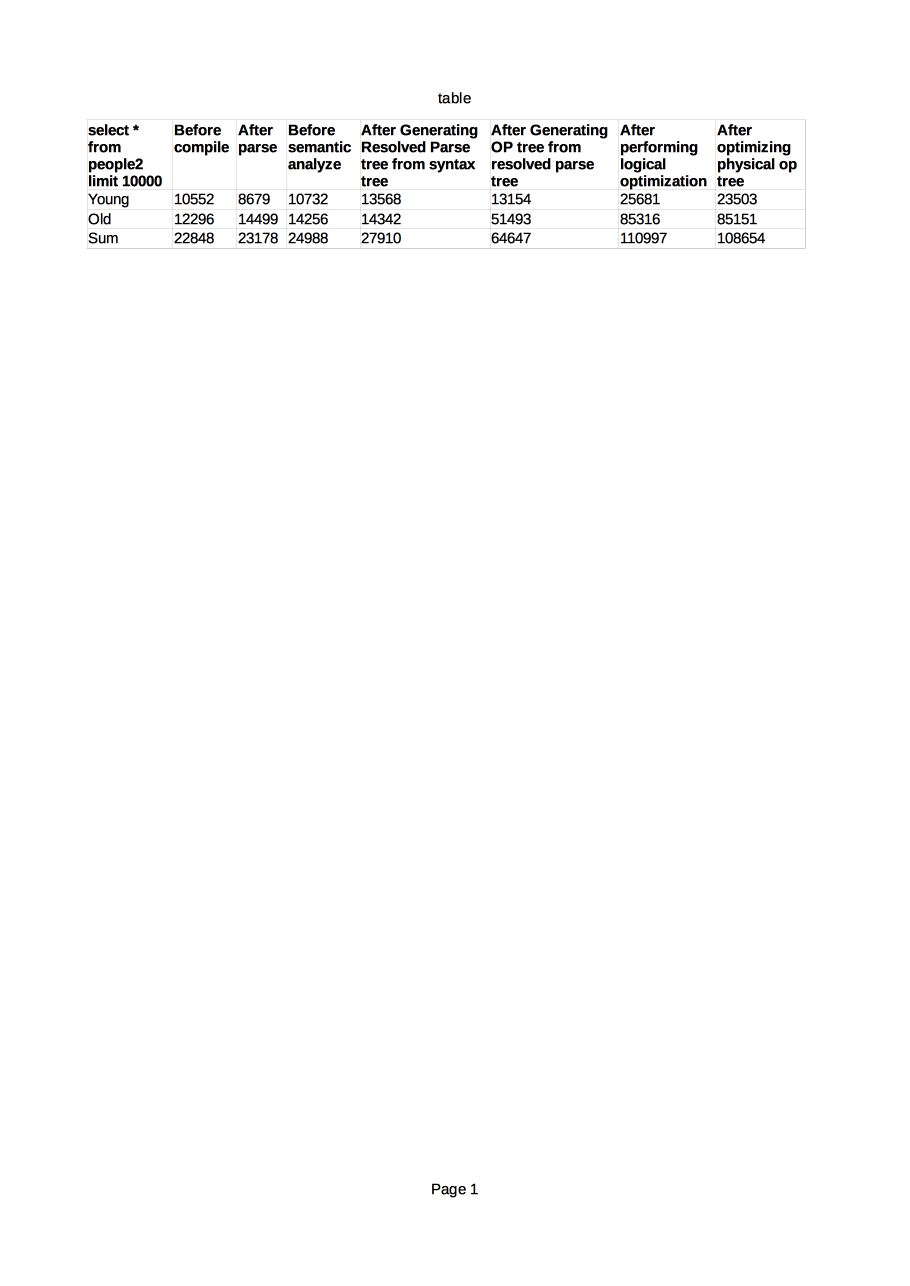
\includegraphics[width=150mm, keepaspectratio]{figures/parse_output.png}
	\centering
	\caption{Sample output of the parsing}
\end{figure}


\subsection{How HiveServer2 uses memory}
I have the code to measure the memory of Hive and get a general picture of the usage at certain phases. With this, I am able to get a better understanding when and why memory goes high. I would like to get an answer to these questions: How does the number of joins increase the memory? Which type of query generates a lot of memory usage: union, group by? If we increase the number of partitions, how it affects the heap size? In this section, these questions will be answered.

The first step is to create a managed table where I will run my queries in the future. Hive faces memory problems when we have a highly partitioned table. I decided that for the first run, 20 000 partitions will be enough. 

The second step was to create queries which will be submitted to Hive. The first question was how the number of joins affects memory? To answer it, I have created queries with an increasing number of joins included. I used self-joins and only increased the number to three. The pattern was clear for only four measures: a simple select query without join operator, and queries with one, two and three. From the output of my parsed CSV file, I generated the following chart that shows the memory increase.

\begin{figure}[H]
	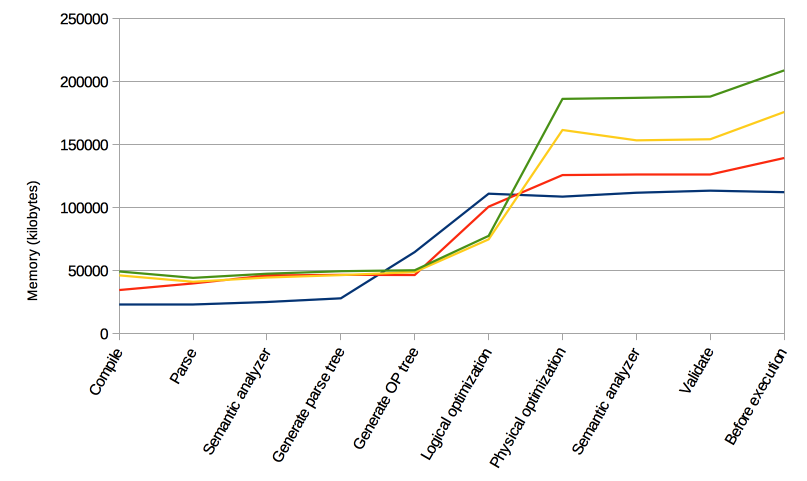
\includegraphics[width=150mm, keepaspectratio]{figures/hs2_joins_memory.png}
	\centering
	\caption{Heap size with increasing number of joins}
\end{figure}

\noindent Queries run with their color in the chart:
\begin{itemize}
	\item select * from tablename (\textcolor{blue}{\rule{2 cm}{2pt} })
	\item select * from tablename t1 join tablename t2 on t1.id=t2.id (\textcolor{orange}{\rule{2 cm}{2pt} })
	\item select * from tablename t1 join tablename t2 on t1.id=t2.id join tablename t3 on t2.id=t3.id (\textcolor{yellow}{\rule{2 cm}{2pt} })
	\item select * from tablename t1 join tablename t2 on t1.id=t2.id join tablename t3 on t2.id=t3.id join tablename t4 on t3.id=t4.id (\textcolor{green}{\rule{2 cm}{2pt} })
\end{itemize}

We can see that the memory change caused by the number of join operators is negligible, only around 20 Megabytes per join. The results were as expected: the memory increased significantly when HiveServer2 connected to the MetaStore and asked for metadata. During physical optimization, Hive loaded metadata to memory including partition metadata. In a highly partitioned table, this size is notable. Although real queries submitted to Hive by users are much more complicated and contains multiple tables, the model will be quite similar: heap memory will rise when metadata is loaded.

I also wanted to see the memory effects of \textit{group by} and  \textit{union all} operations. I ran 5 more queries including these but did not find anything notable. The pattern remained the same: see the chart below. 

\begin{figure}[H]
	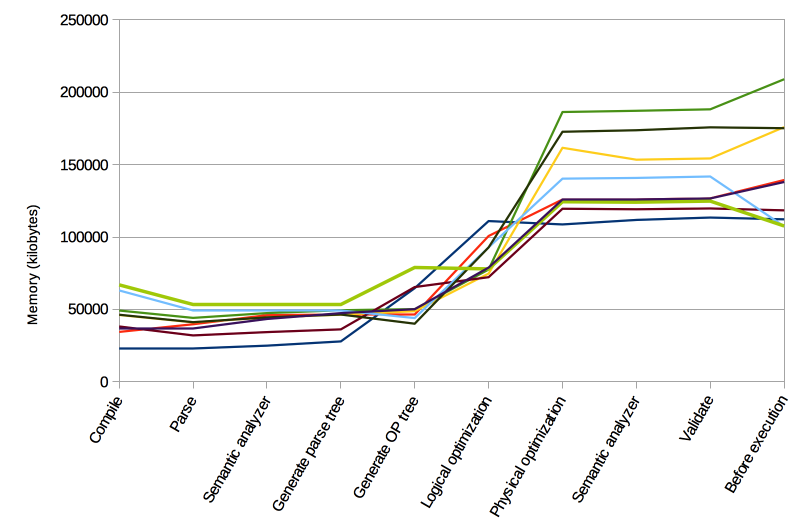
\includegraphics[width=150mm, keepaspectratio]{figures/hs2_memory.png}
	\centering
	\caption{Heap size when running various type of queries}
\end{figure}

I came to the conclusion that for a single connection to HiveServer2, the most important factor that increases heap size is the number of partitions in tables, so I decided to continue my investigation in that area. 

\subsection{Memory consumption of partitions}
A well-known issue in Hive is, if we have a highly partitioned table, the memory goes really high in HiveServer2. As a first step, I wanted to recreate the issue. I created tables with an increasing number of partitions: 200, 2000, 5000, 20000 and 100000 partitions. For each table, I executed the same query which contains a simple select with a self-join. During this, I measured the memory and created a heap dump after the semantic analyzer phase of the compilation. At this stage, the partitions are already loaded so I can analyze how much these objects exactly reserve. To get this information, I analyzed the heap dumps with VisualVM and filtered for the Partition objects. The pattern we can observe was as expected, but I the size of the heap reserved by these objects were smaller than I previously anticipated.

\noindent From the heap dumps I have found that mainly three kind of objects reserve the memory due to partitions, so I will focus on these objects: 
\begin{enumerate}
	\item hive.ql.metadata.Partitions
	\item hive.metastore.api.Partition
	\item hive.ql.plan.PartitionDesc
\end{enumerate}

\begin{table}[H]
	\begin{tabular}{|l|l|l|l|l|}
		\hline
		& \textbf{\begin{tabular}[c]{@{}l@{}}ql.metadata.\\ Partitions\end{tabular}} & \textbf{\begin{tabular}[c]{@{}l@{}}metastore.api.\\ Partition\end{tabular}} & \textbf{\begin{tabular}[c]{@{}l@{}}ql.plan.\\ PartitionDesc\end{tabular}} & \textbf{Sum} \\ \hline
		\textbf{200 partitions}    & 300 Kb                                                                     & 288 Kb                                                                      & 108 Kb                                                                    & 696 Kb       \\ \hline
		\textbf{2000 partitions}   & 3057 Kb                                                                    & 2946 Kb                                                                     & 1110 Kb                                                                   & 7113 Kb      \\ \hline
		\textbf{5000 partitions}   & 7988 Kb                                                                    & 7709 Kb                                                                     & 2793 Kb                                                                   & 18490 Kb     \\ \hline
		\textbf{20000 partitions}  & 29999 Kb                                                                   & 28879 Kb                                                                    & 3173 Kb                                                                   & 62051 Kb     \\ \hline
		\textbf{100000 partitions} & 165002 Kb                                                                  & 158841 Kb                                                                   & 60531 Kb                                                                  & 384374 Kb    \\ \hline
	\end{tabular}
\caption{Memory of partitions}
\end{table}

\begin{figure}[H]
	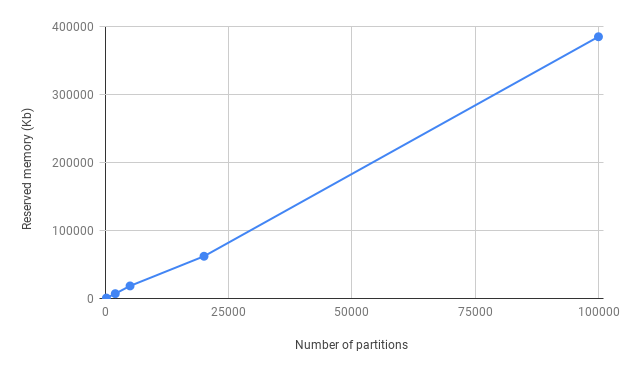
\includegraphics[width=150mm, keepaspectratio]{figures/partitions_chart.png}
	\centering
	\caption{Reserved memory by partitions}
\end{figure}

As we see, for 100.000 partitions the reserved memory is aroung 385 Megabytes. Before taking the samples, I expected higher memory consumption. However, with a little investigation I found that the memory waste around partitions was already somewhat decreased \cite{hive-partitions}. PartitionDesc objects has a java.util.Properties field. These Properties fields in the PartitionDesc most often are the same. Interning these saves a big amount of memory. In a later section, I will write more about the interning solution because it gave me an idea to fix another memory related issue.

However the memory reserved by partitions is still high enough, so I decided to take a look at the heap dumps and try to find wastes or problems that affects memory usage.